\chapter{Evaluatie}\label{sec:evaluatie}
We hebben software ontworpen die een interne voorstelling heeft voor de informatie bevat in een klassediagram en een stel bijhorende sequentiediagrammen. De software kan die interne voorstelling vertalen naar een FO($\cdot$)-theorie opgesteld volgens de regels bekomen in hoofdstukken \ref{sec:consistentie} en \ref{sec:gedrag}. Het was ook gepland om voor voorstellingen van klassediagrammen en sequentiediagrammen in XML een vertaler naar onze interne voorstelling te voorzien, maar door tijdsgebrek is deze vertaler niet ge\"implementeerd.

In dit hoofdstuk ontwerpen we een klassediagram en sequentiediagrammen waarmee we het spel Nim modelleren zonder gebruik te maken van de nieuwe instructies uit sectie \ref{sec:newlang}. We vertalen die diagrammen dan manueel naar onze interne voorstelling en laten een FO($\cdot$)-theorie genereren. Voor de uitvoertheorie beoordelen we de volgende zaken:

\begin{itemize}
	\item Hoe gemakkelijk het is om tot een ontwerp te komen.
	\item Of we het spel kunnen spelen met de uitvoertheorie.
	\item Of we bepaalde gewenste eigenschappen kunnen verifi\"eren.
	\item Performantie: Tijd- en geheugengebruik. We zetten in onze IDP-bestanden \textit{stdoptions.verbosity.groundingstats} op 1 om IDP het tijdgebruik en de grootte van de \textit{grounding}\cite{DeCatBroes2014PLaa} te laten rapporteren. Aangezien onze gebruikte versie van IDP, namelijk 3.7.0, voor progressie\"inferentie geen nuttige statistieken geeft over \textit{grounding}-grootte, gebruiken we voor de evaluatie van de speelbaarheid in de plaats het gebruik aan virtueel geheugen op bepaalde tijdstippen.
\end{itemize}

\section{Ontwerp}

Figuur \ref{fig:nim-cd} bevat het klassediagram voor ons ontwerp van Nim.

De klasse \textit{Game} stelt het concept van een spel voor. \textit{p1Win} geeft aan of speler 1 heeft gewonnen en \textit{gameFinished} geeft aan of het spel volledig gespeeld is. \textit{allHeapsEmpty()} vraagt op of alle \textit{Heap}s leeg zijn. \textit{takeTurn()} doet een speler zijn beurt spelen. \textit{play(boolean)} is de methode die het verloop van het spel regelt.

De klasse \textit{Heap} stelt stapels van objecten voor. \textit{numObjects} is het aantal objecten dat een stapel bevat. \textit{isEmpty()} geeft aan of de stapel leeg is en \textit{take(int)} neemt een aantal objecten weg van een stapel.

Figuren \ref{fig:nim-take}, \ref{fig:nim-play}, \ref{fig:nim-allHeapsEmpty}, \ref{fig:nim-isEmpty} en \ref{fig:nim-takeTurn} bevatten de sequentiediagrammen die het gedrag van hun bijhorende methodes modelleren.

Diagram \ref{fig:nim-take} berekent hoeveel objecten er nog overblijven op een stapel gegeven een aantal objecten om weg te nemen van de stapel. Als het verschil kleiner is dan nul, wordt de teller op nul gezet.

Diagram \ref{fig:nim-play} bepaalt eerst of alle stapels leeg zijn. Zo ja, is het spel voorbij en is de speler die nu aan beurt is de winnaar. Zo nee, speelt de huidige speler een ronde en geeft de beurt door aan de andere speler.

Diagram \ref{fig:nim-allHeapsEmpty} vraagt aan alle stapels om de beurt of ze leeg zijn. Als het een stapel tegenkomt die niet leeg is, is het antwoord meteen nee. Als het enkel stapels tegenkomt die leeg zijn, is het antwoord ja.

Diagram \ref{fig:nim-isEmpty} antwoordt ja als de stapel leeg is en nee als de stapel niet leeg is.

Diagram \ref{fig:nim-takeTurn} vraagt aan de speler van welke stapel hij objecten wil nemen. Er wordt vanaf nul geteld, dus moet hij nul antwoorden als hij de eerste stapel wil selecteren. Als de geselecteerde stapel leeg is, wordt er opnieuw gevraagd om een stapel te selecteren. Als de speler een stapel heeft gekozen die niet leeg is, moet hij kiezen om minstens \'e\'en en maximaal het aantal objecten dat nog overblijft op de stapel weg te nemen.

Appendix \ref{code:nim-eval} bevat het IDP-bestand met de automatisch gegenereerde uitvoertheorie voor deze diagrammen.

\begin{figure}[htp]
	\centering
	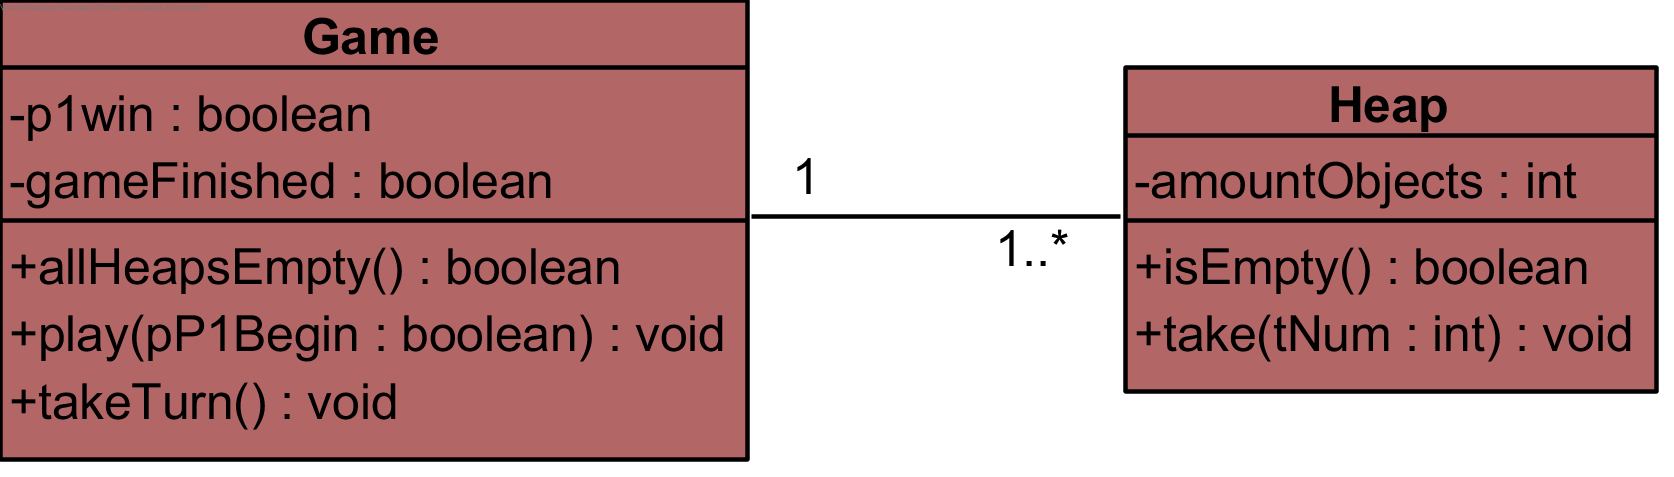
\includegraphics[width=0.75\textwidth]{chap-evaluatie/ClassDiagram1.png}
	\caption{Klassediagram voor Nim}
	\label{fig:nim-cd}
\end{figure}

%\begin{landscape}
%	\newpage
%	\thispagestyle{plain}
%	\begin{figure}-
%		\centering
%		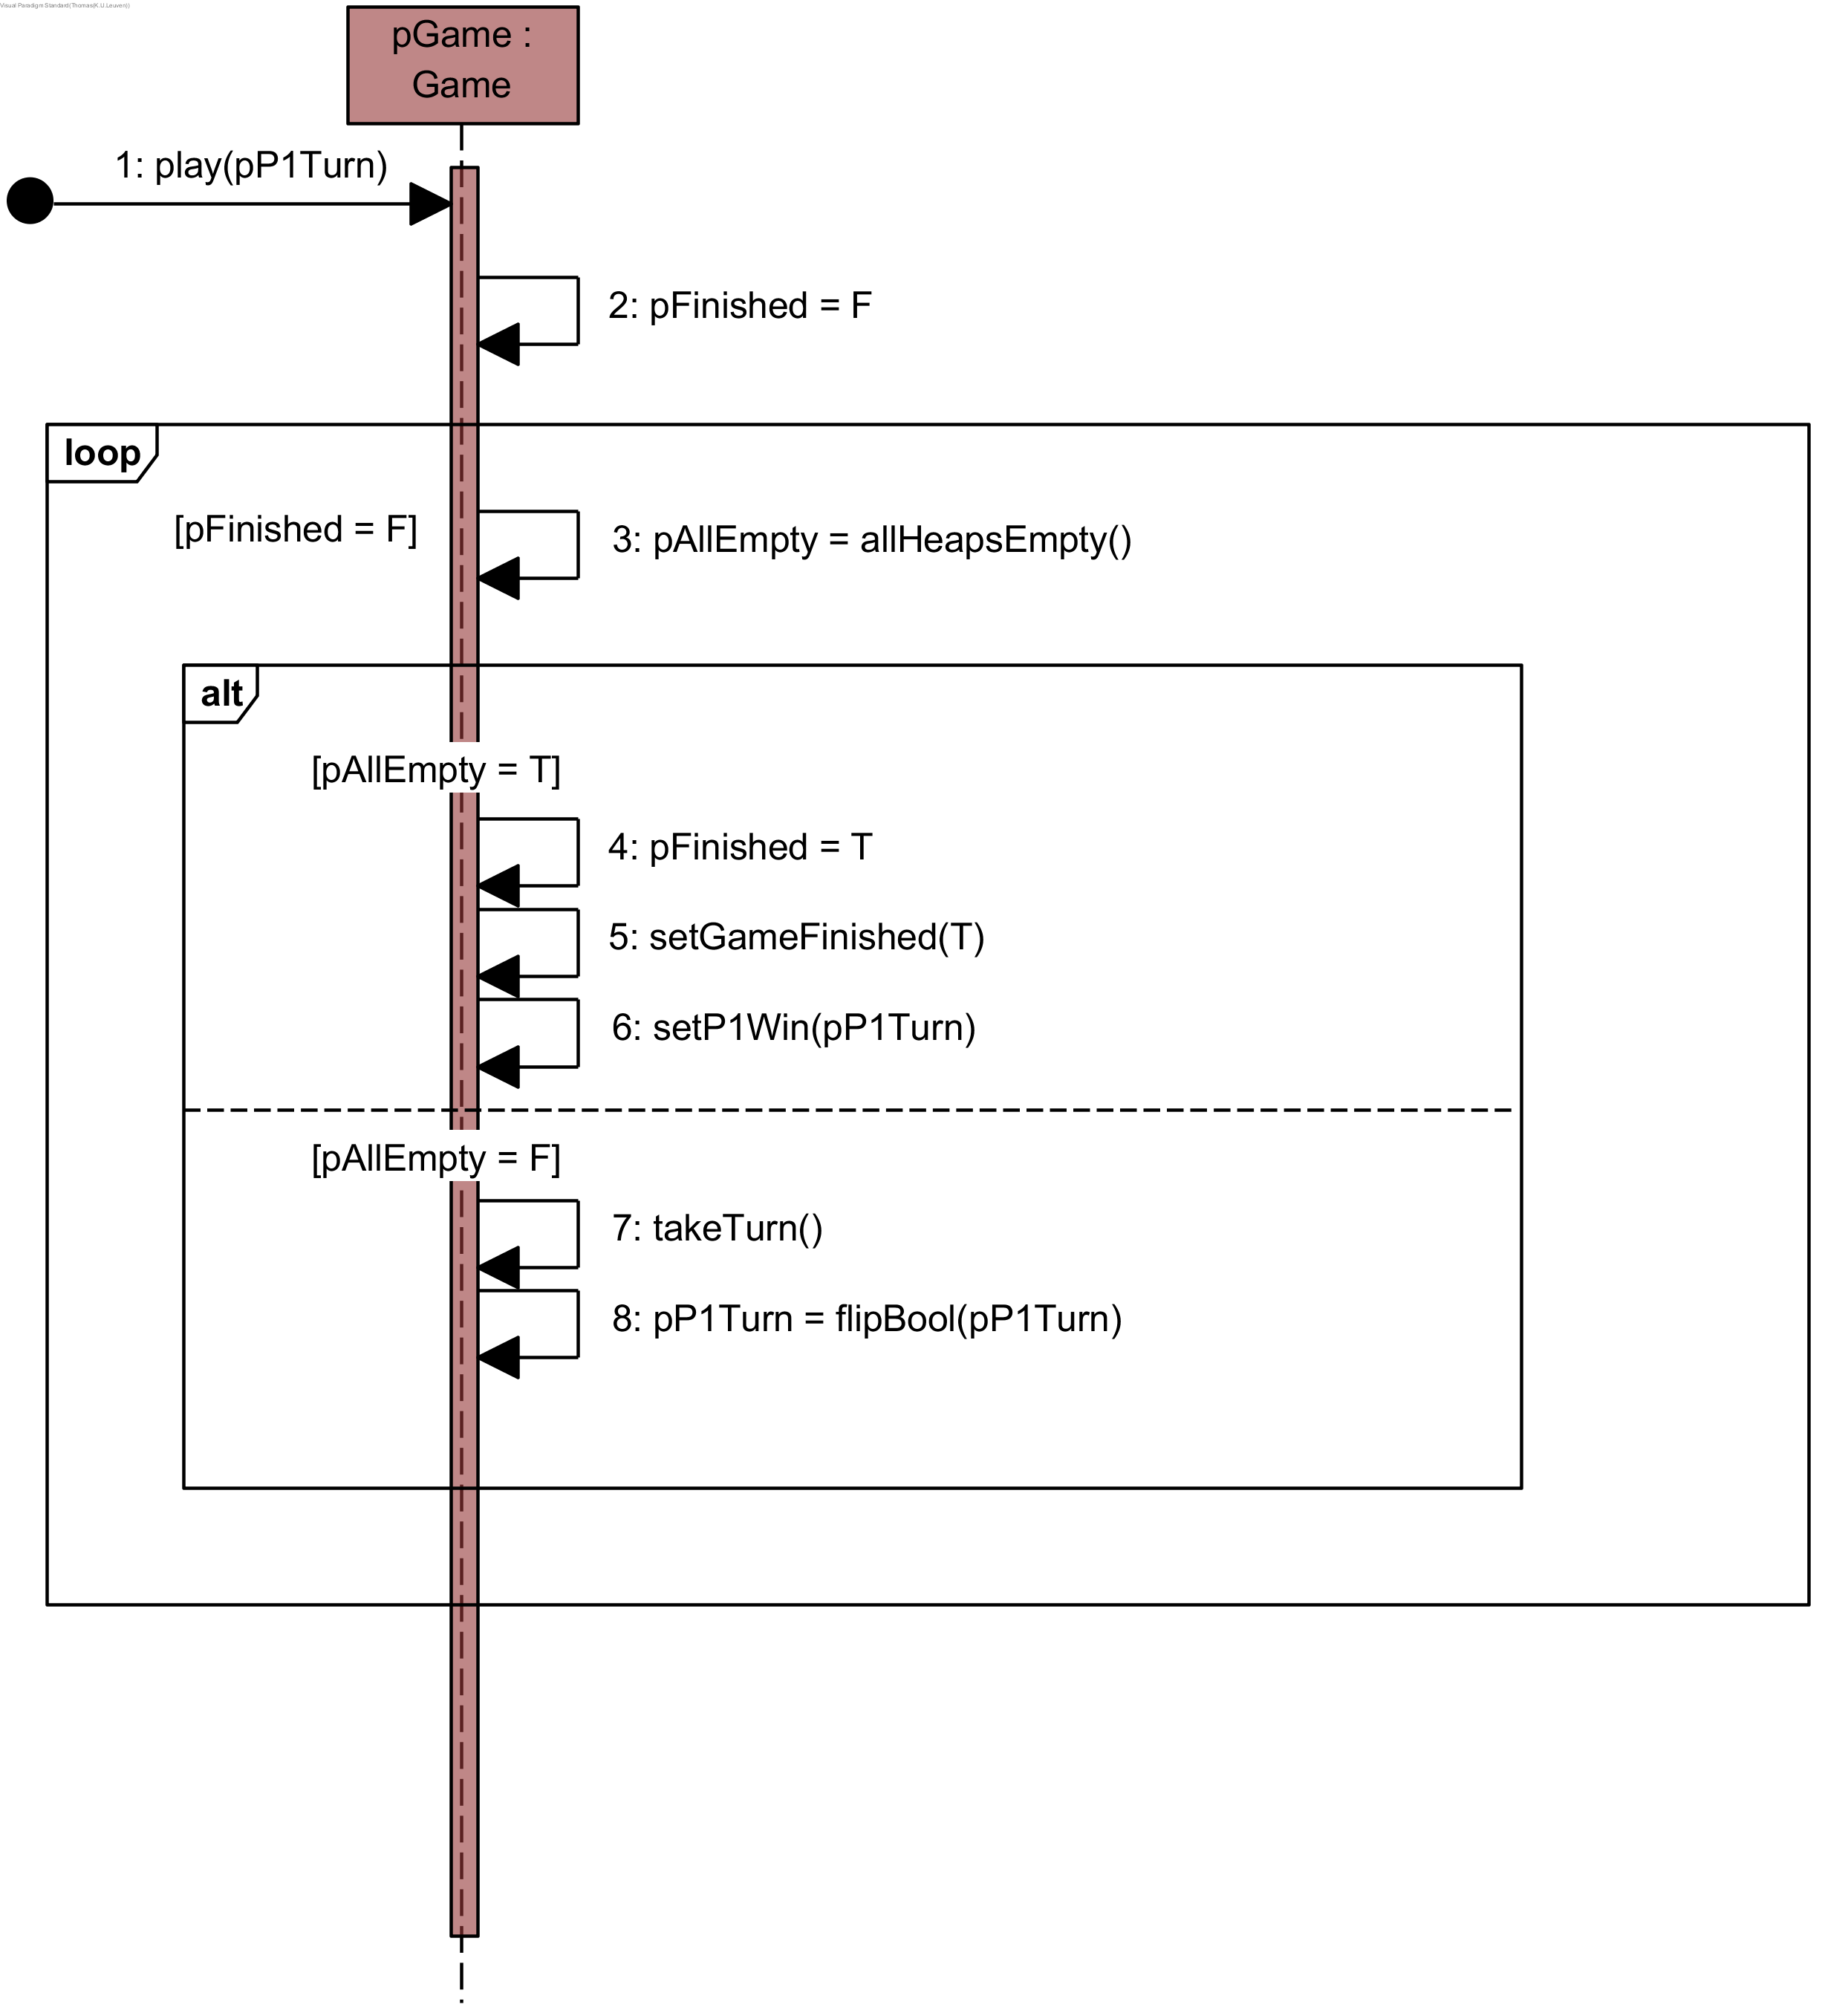
\includegraphics[width=0.4\textwidth]{chap-evaluatie/play.png}
%		\caption{Sequentiediagram voor play()}
%		\label{fig:nim-play}
%	\end{figure}
%	\begin{figure}
%		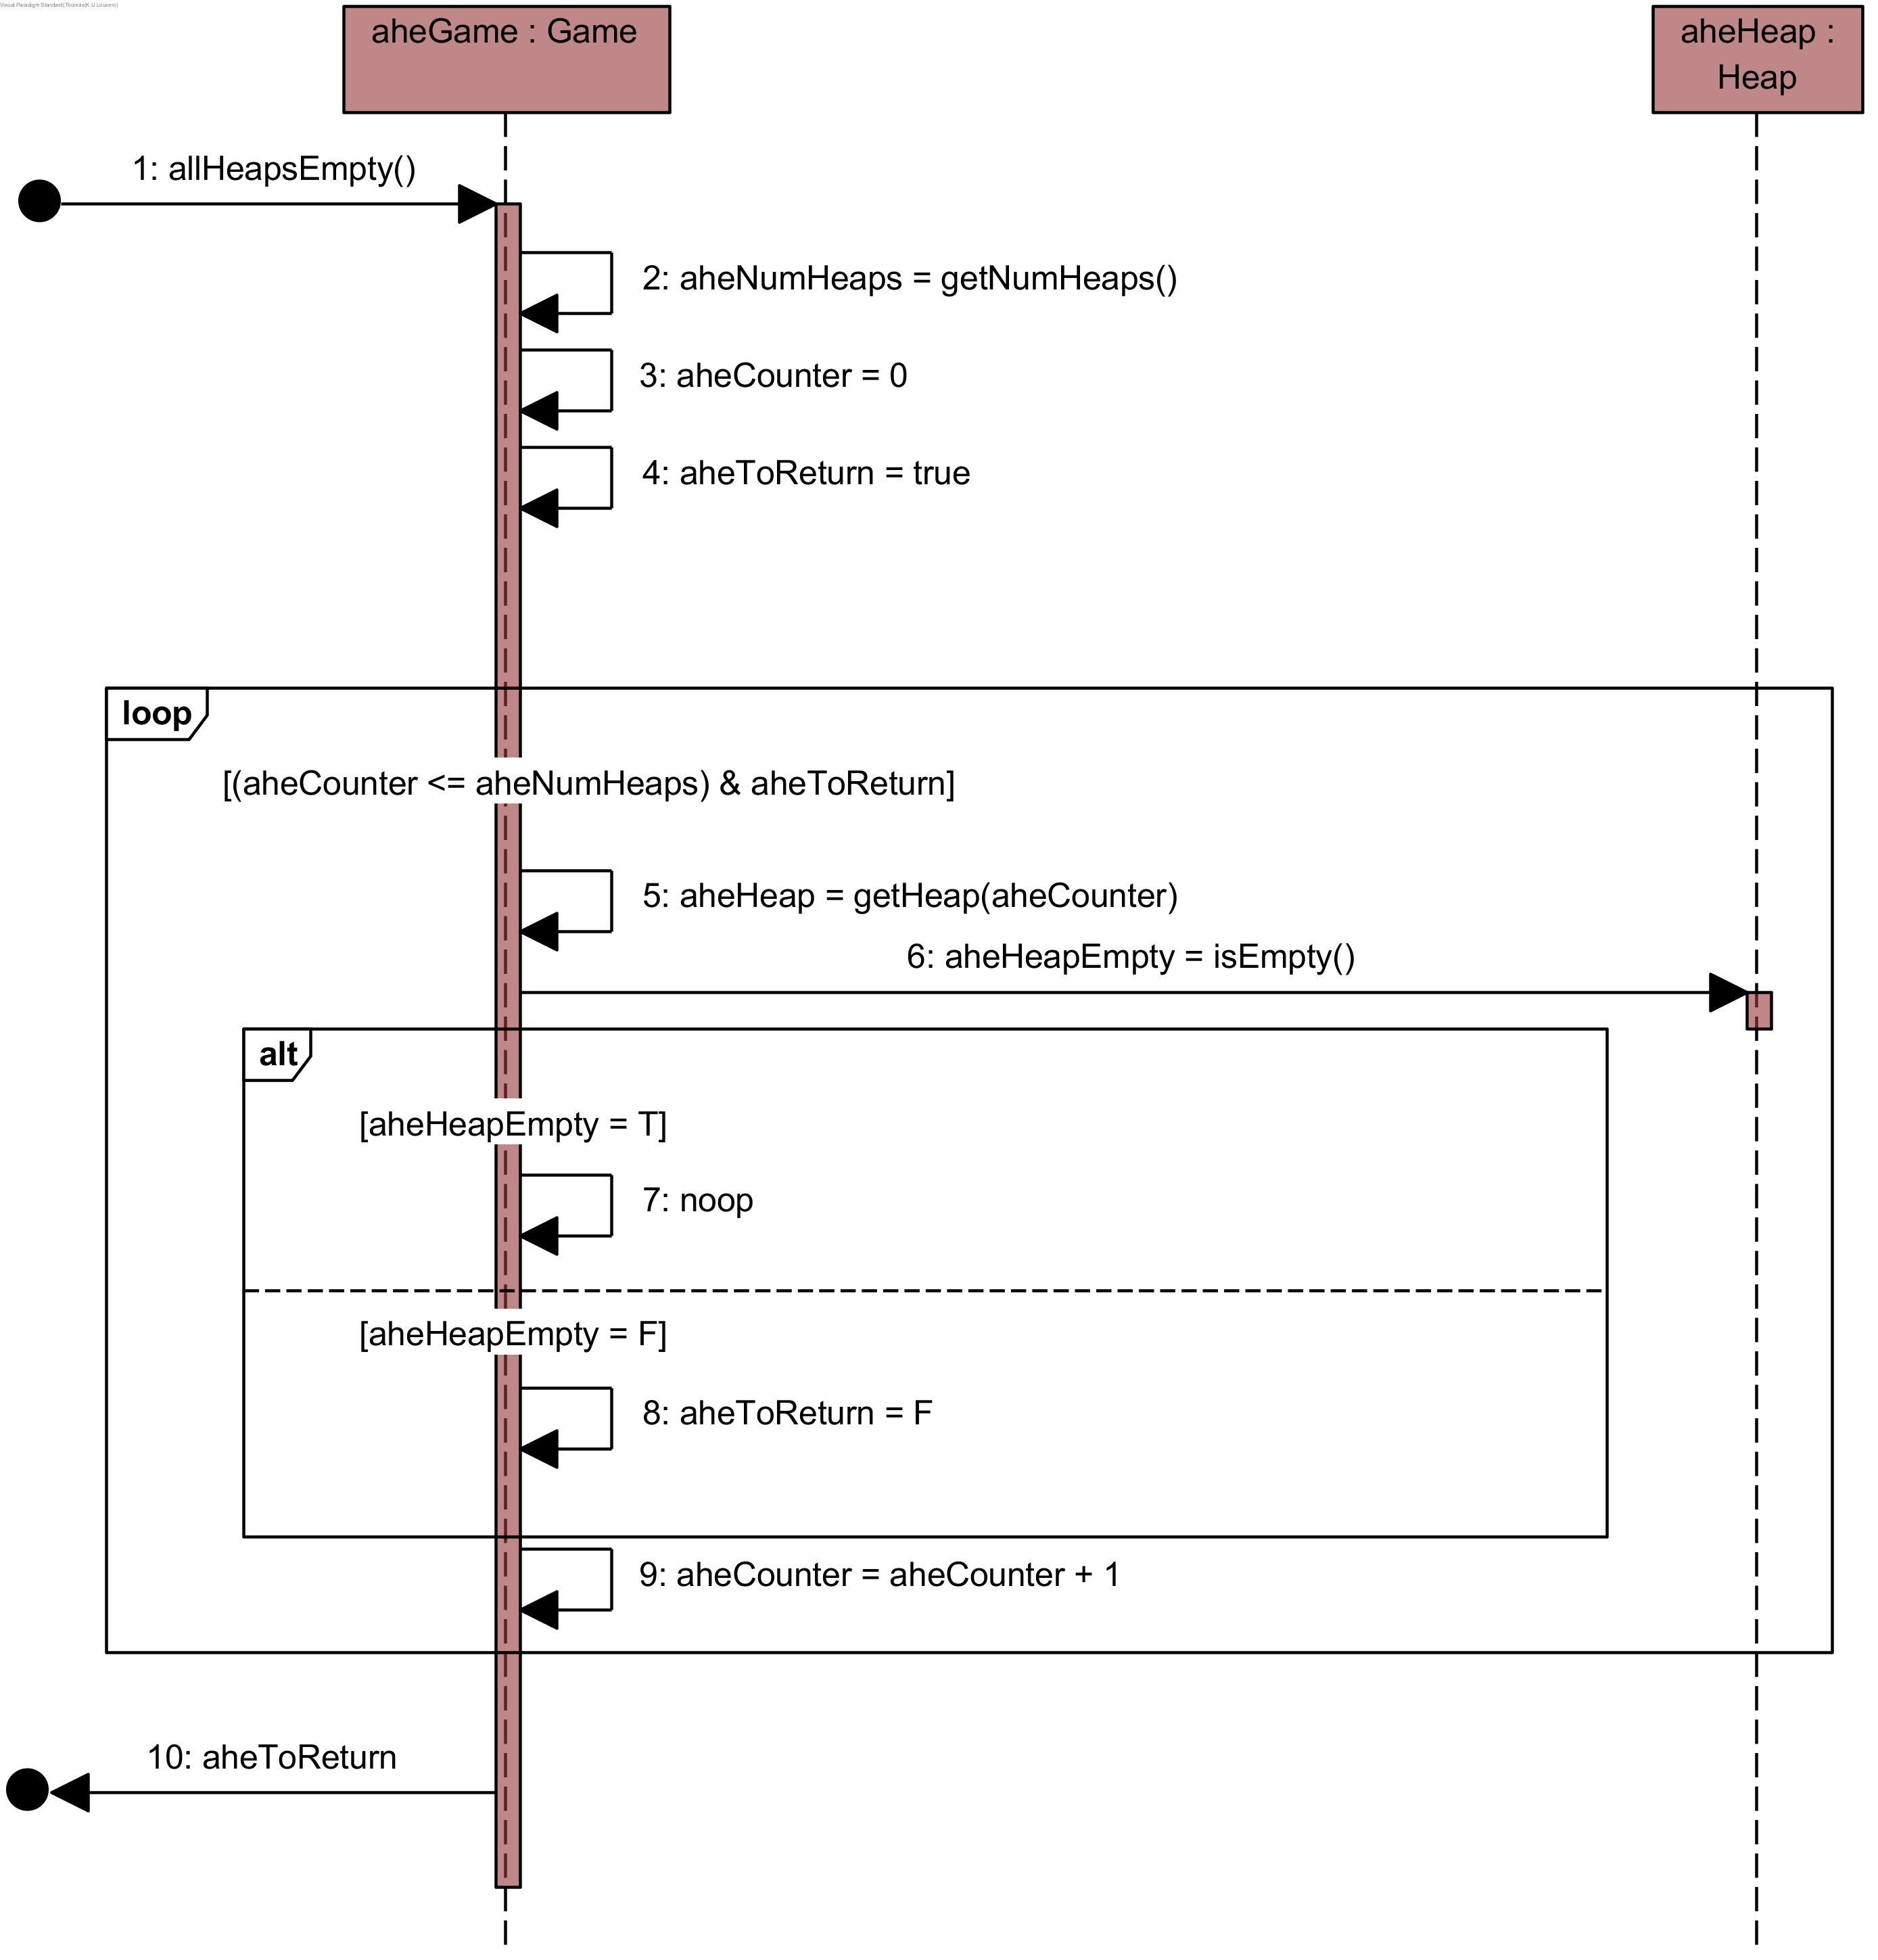
\includegraphics[width=0.75\textwidth]{chap-evaluatie/allHeapsEmpty.png}
%		\caption{Sequentiediagram voor allHeapsEmpty()}
%		\label{fig:nim-allHeapsEMpty}
%	\end{figure}
%\end{landscape}
\afterpage{
\begin{landscape}
	\newpage
	\thispagestyle{empty}
	\begin{figure}
		%\vspace*{-0.5cm}
		\begin{subfigure}{\textwidth}
			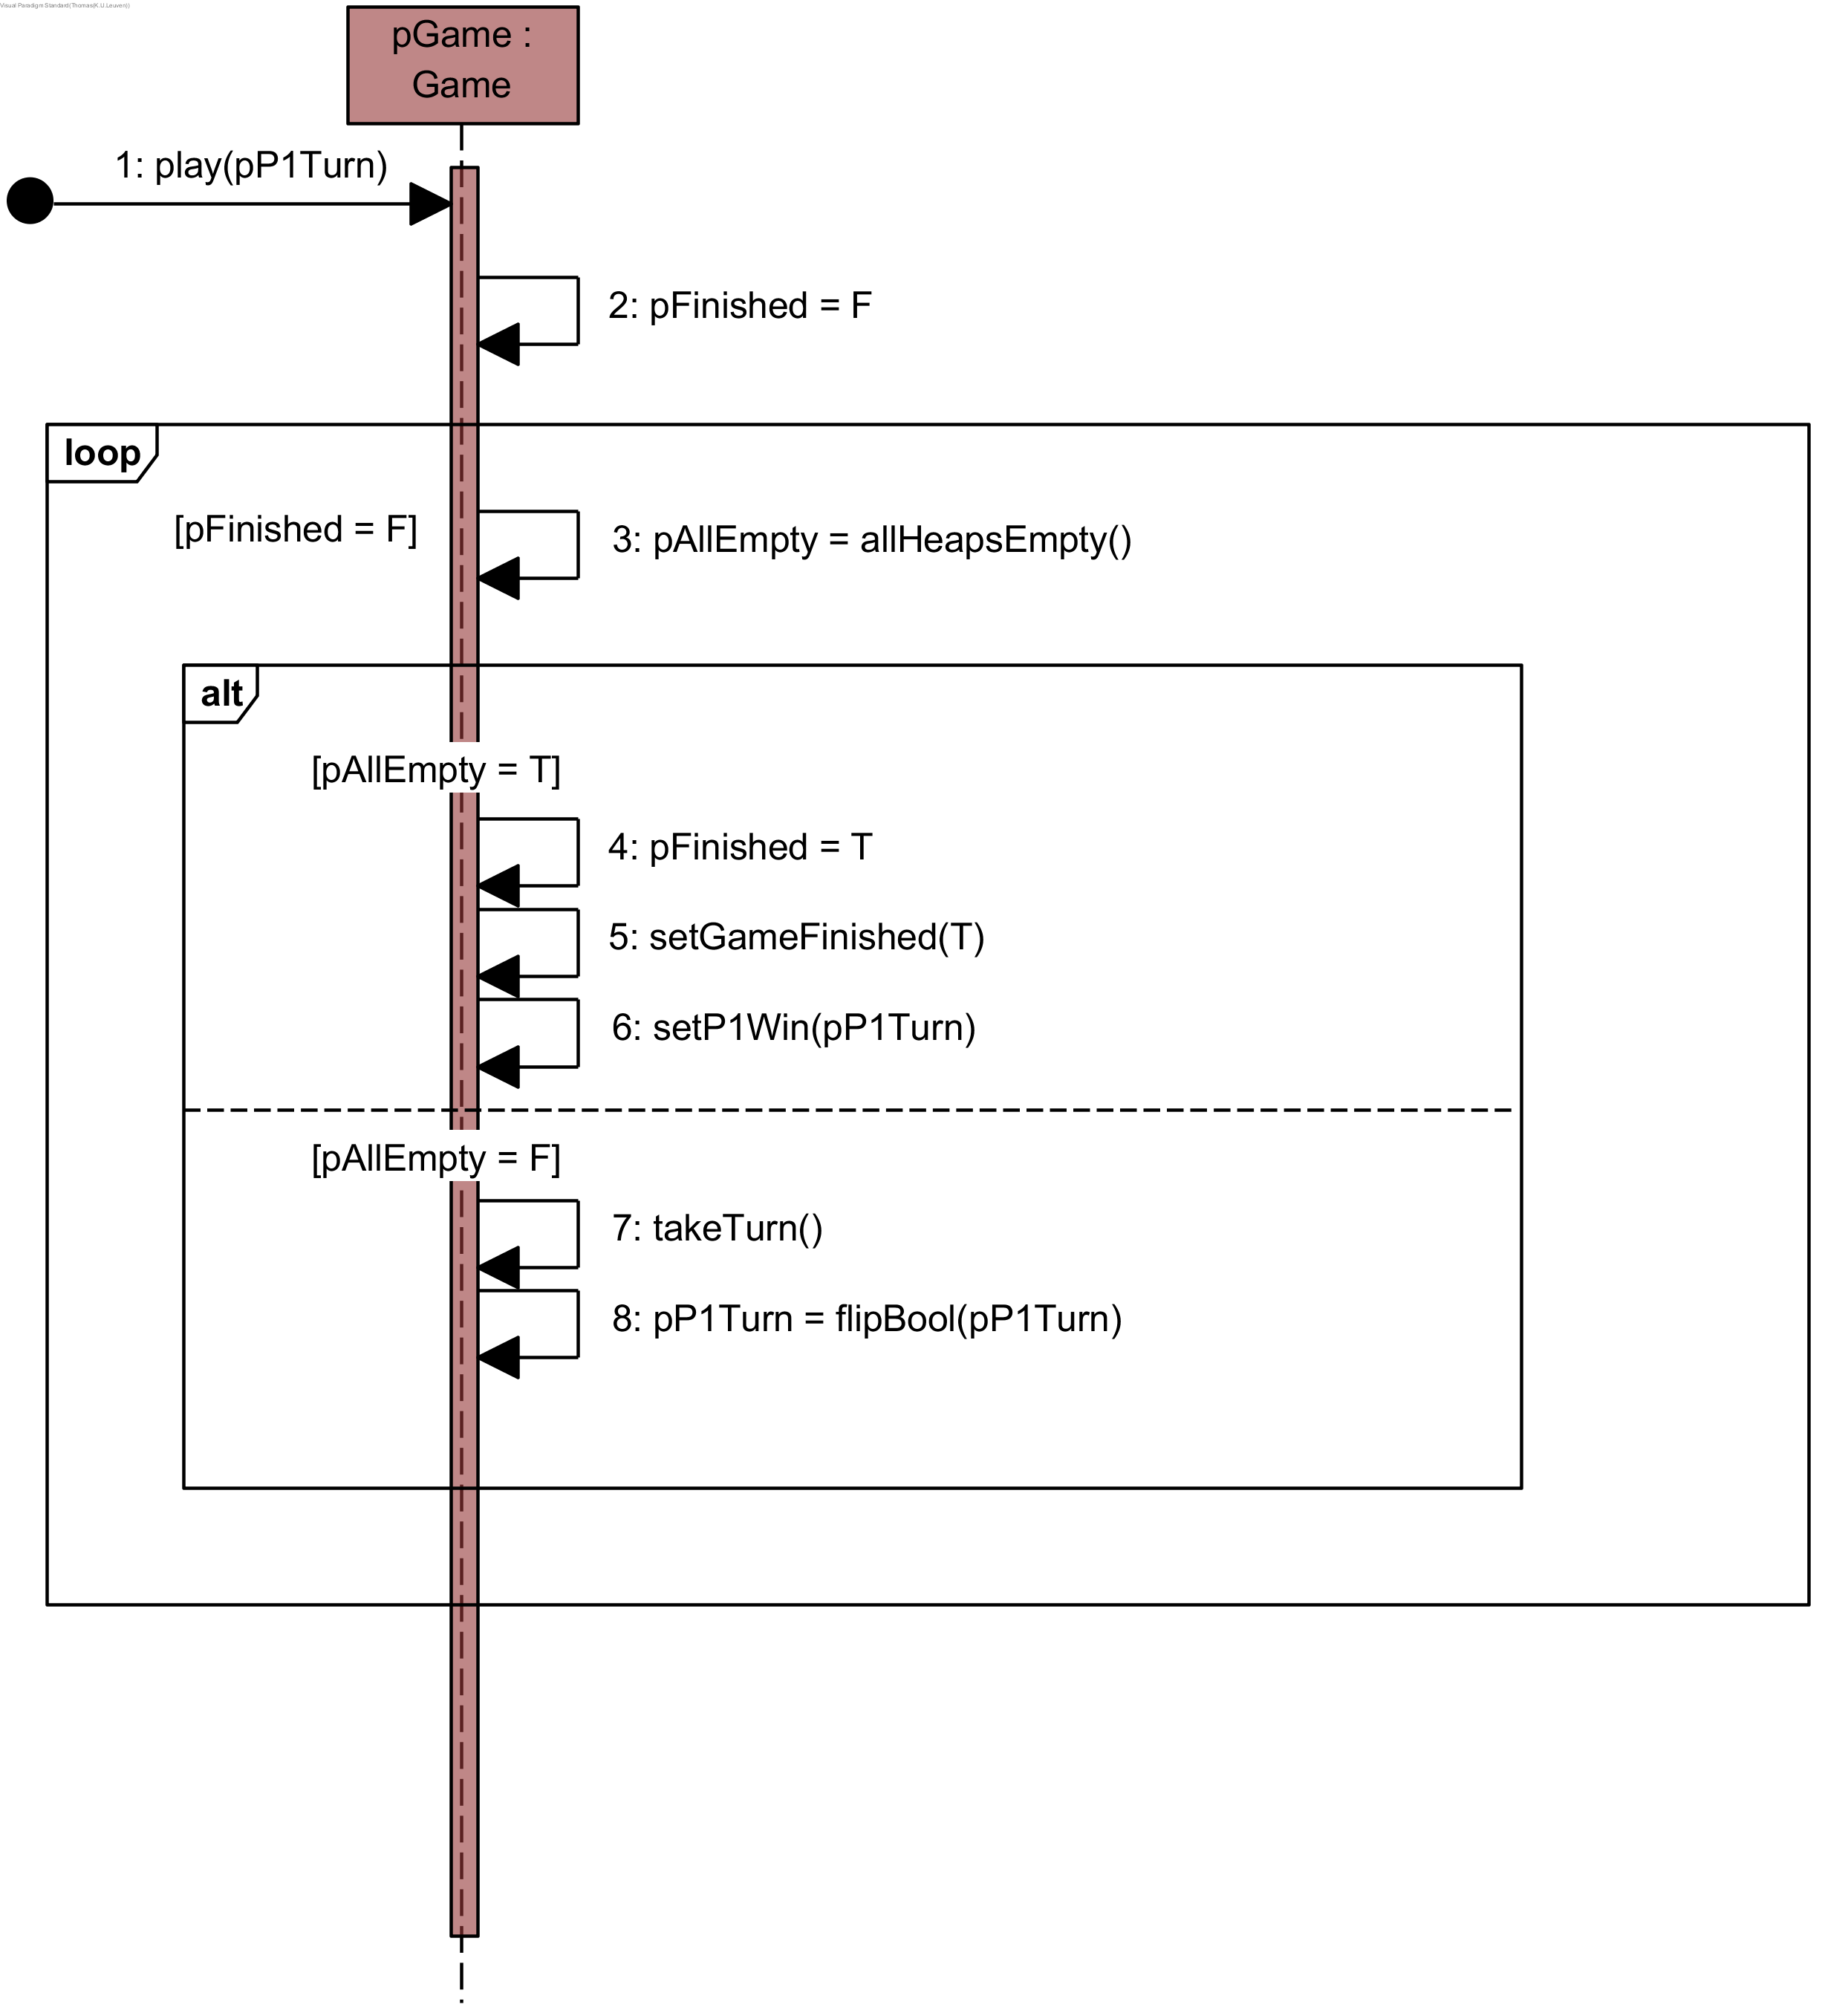
\includegraphics[width=0.8\textwidth]{chap-evaluatie/play.png}
			\caption{Sequentiediagram voor \textit{play(boolean)}}
			\label{fig:nim-play}
		\end{subfigure}%
		\begin{subfigure}{\textwidth}
			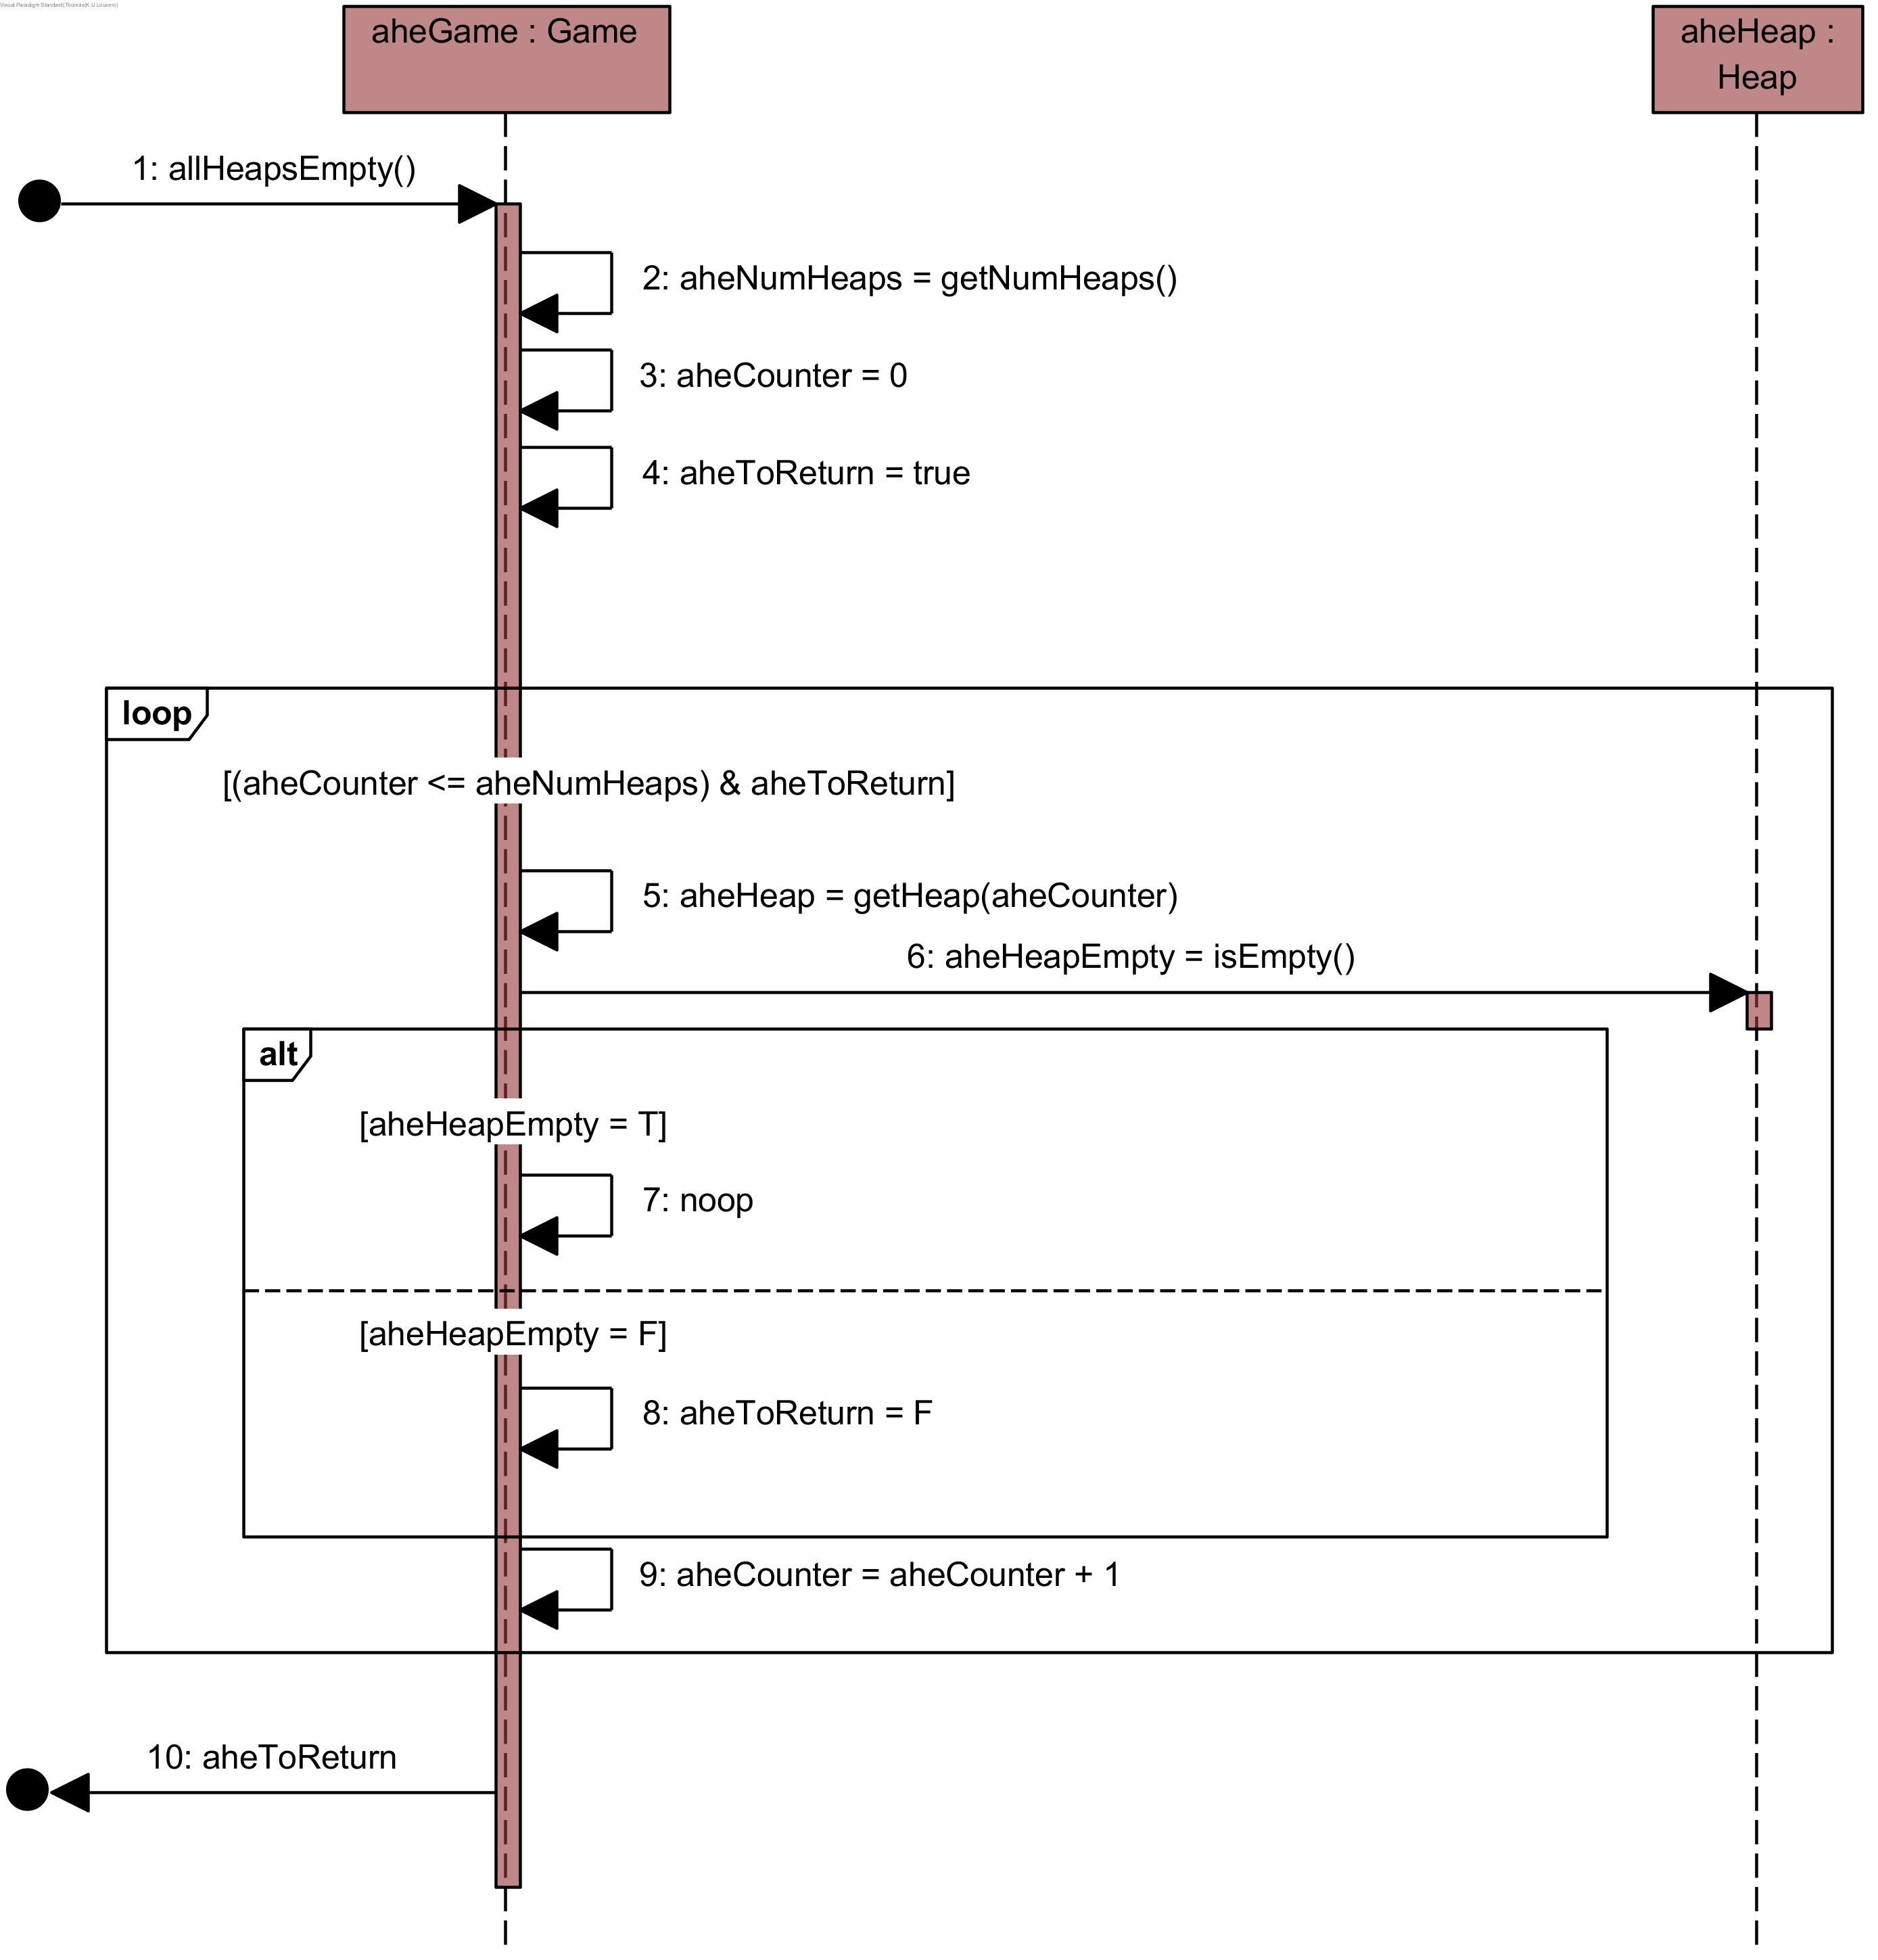
\includegraphics[width=0.8\textwidth]{chap-evaluatie/allHeapsEmpty.png}
			\caption{Sequentiediagram voor \textit{allHeapsEmpty()}}
			\label{fig:nim-allHeapsEmpty}
		\end{subfigure}
		\caption{Sequentiediagrammen voor \textit{play(boolean)} en \textit{allHeapsEmpty()}}
		\label{fig:nim-play-ahe}
	\end{figure}
\end{landscape}
}
\afterpage{
\clearpage
\begin{landscape}
	\newpage
	\thispagestyle{empty}
	
	\begin{figure}
		\begin{subfigure}{\textwidth}
			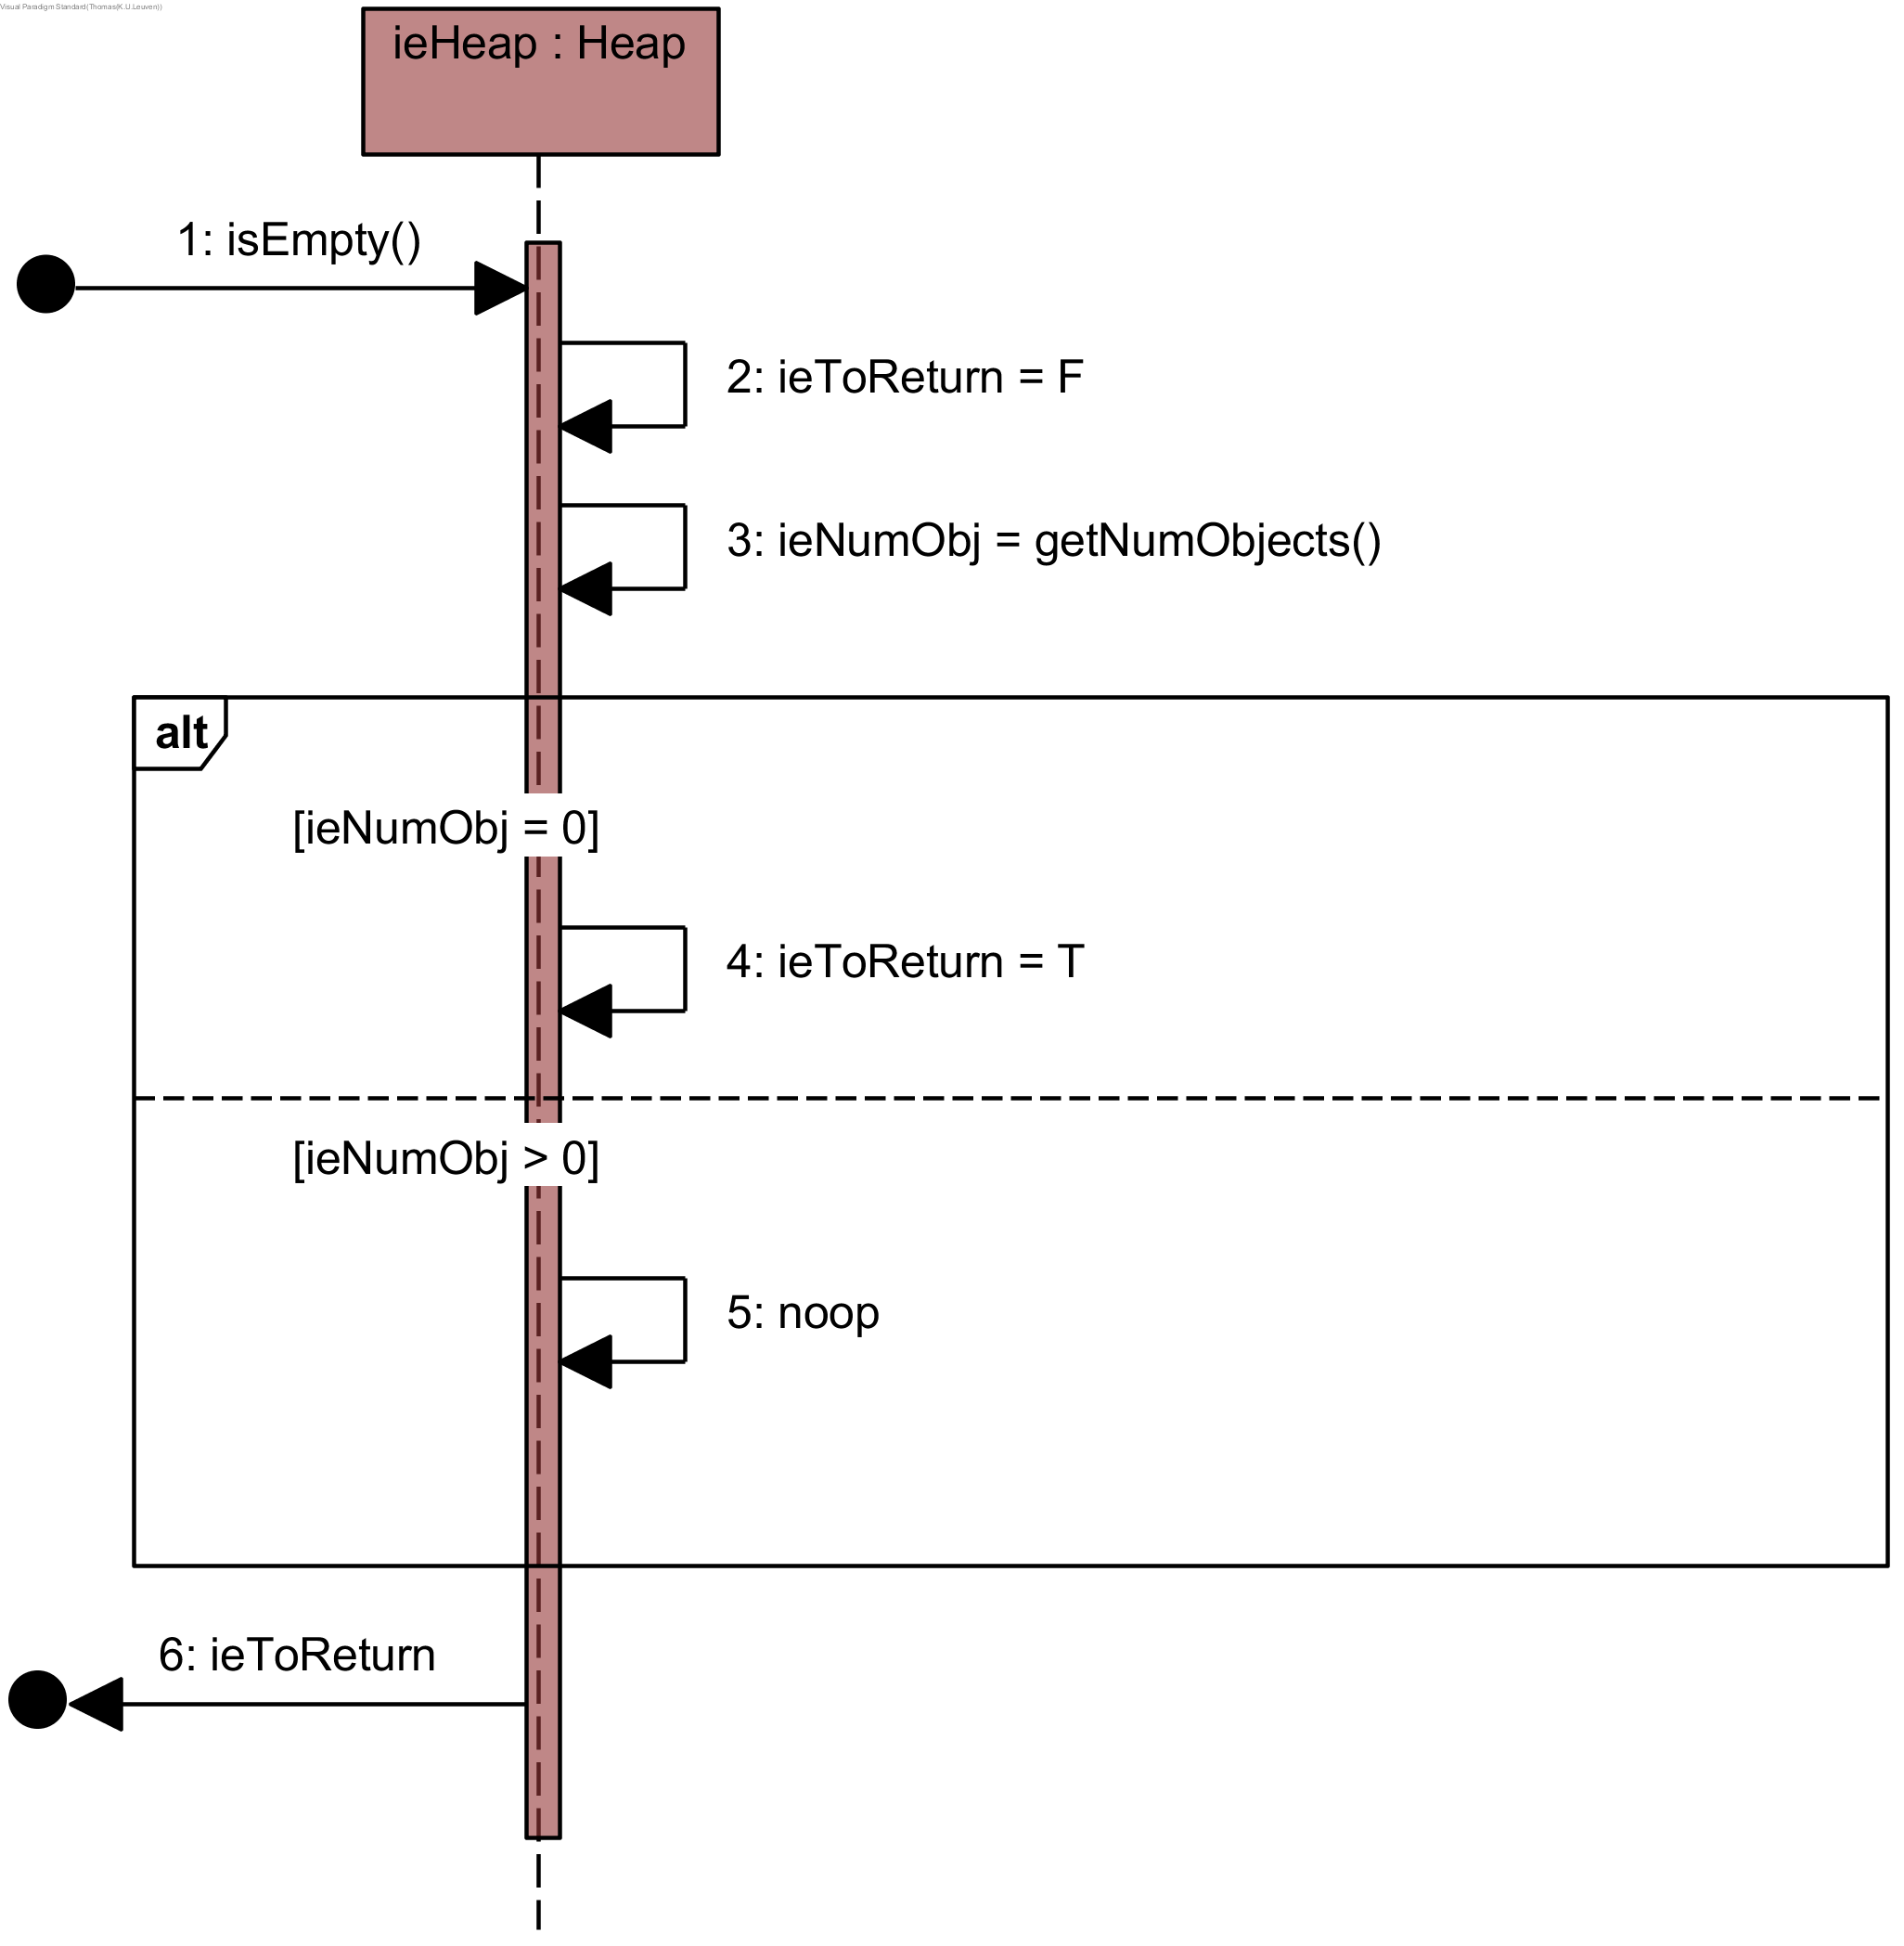
\includegraphics[width=0.75\textwidth]{chap-evaluatie/isEmpty.png}
			\caption{Sequentiediagram voor \textit{isEmpty()}}
			\label{fig:nim-isEmpty}
		\end{subfigure}%
		\begin{subfigure}{\textwidth}
			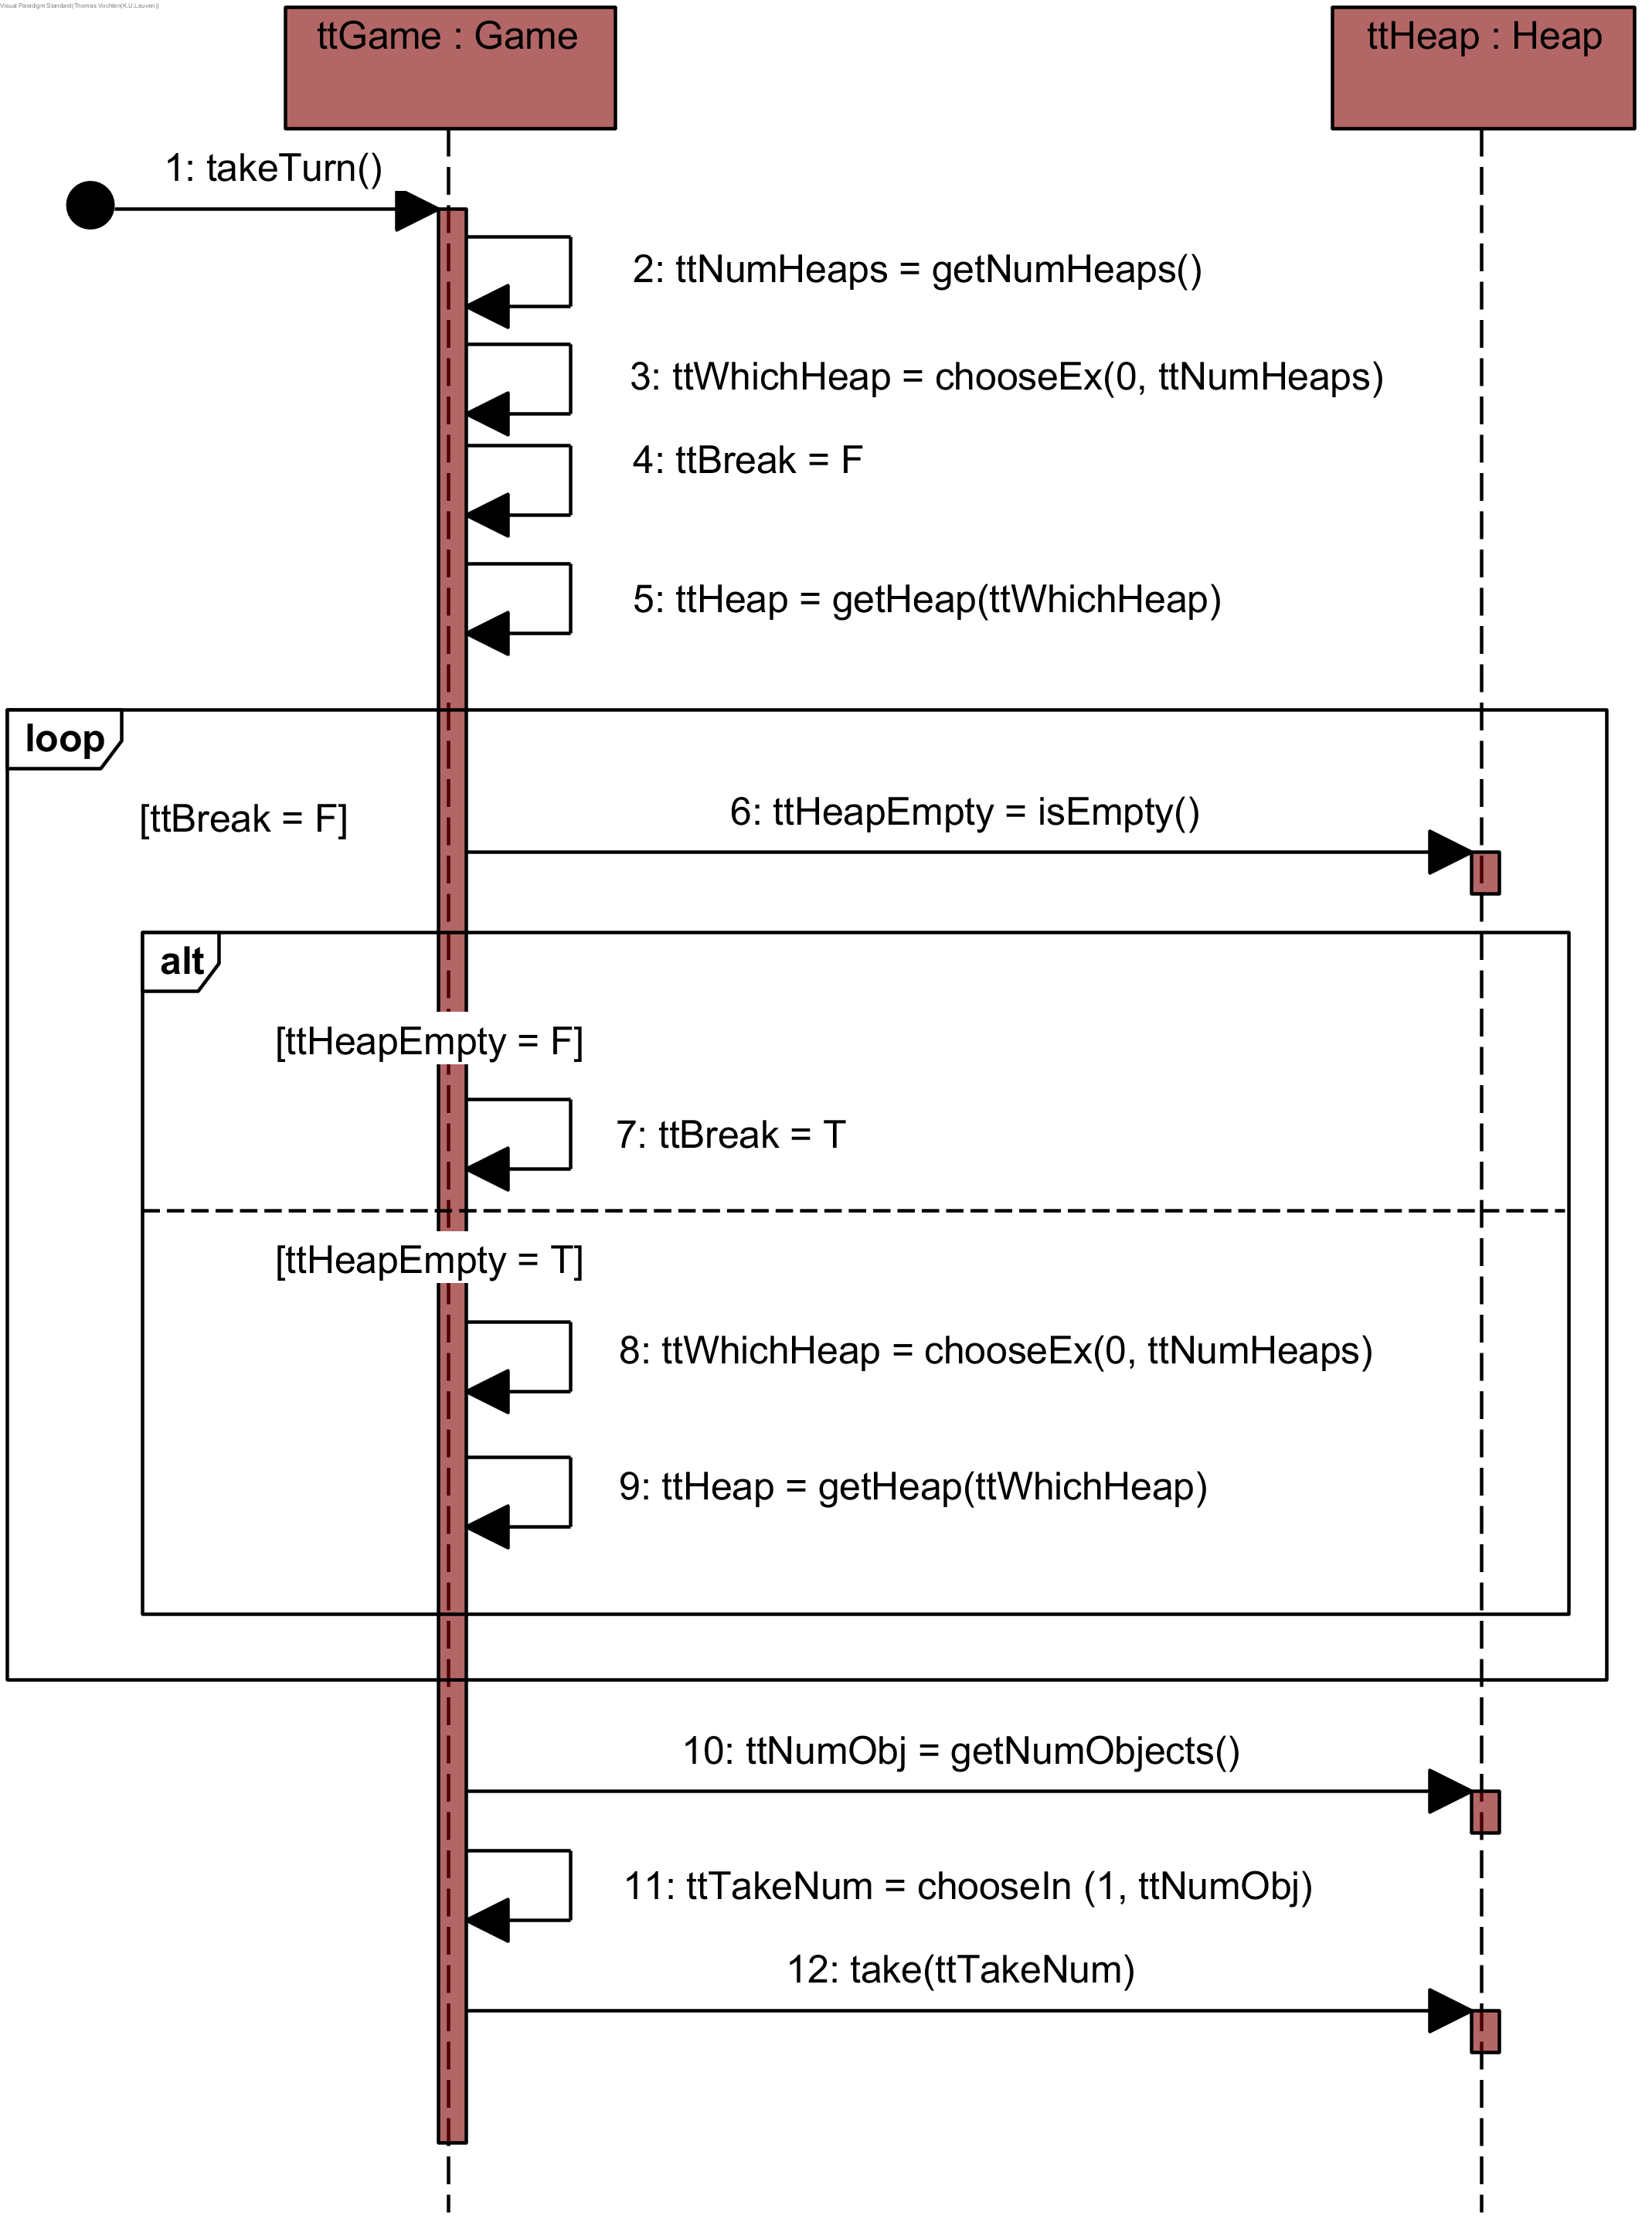
\includegraphics[width=0.8\textwidth]{chap-evaluatie/takeTurn.png}
			\caption{Sequentiediagram voor \textit{takeTurn()}}
			\label{fig:nim-takeTurn}
		\end{subfigure}
		\caption{Sequentiediagrammen voor \textit{isEmpty()} en \textit{takeTurn()}}
		\label{fig:nim-isempty-tt}
	\end{figure}
\end{landscape}
}

\begin{figure}[htp]
	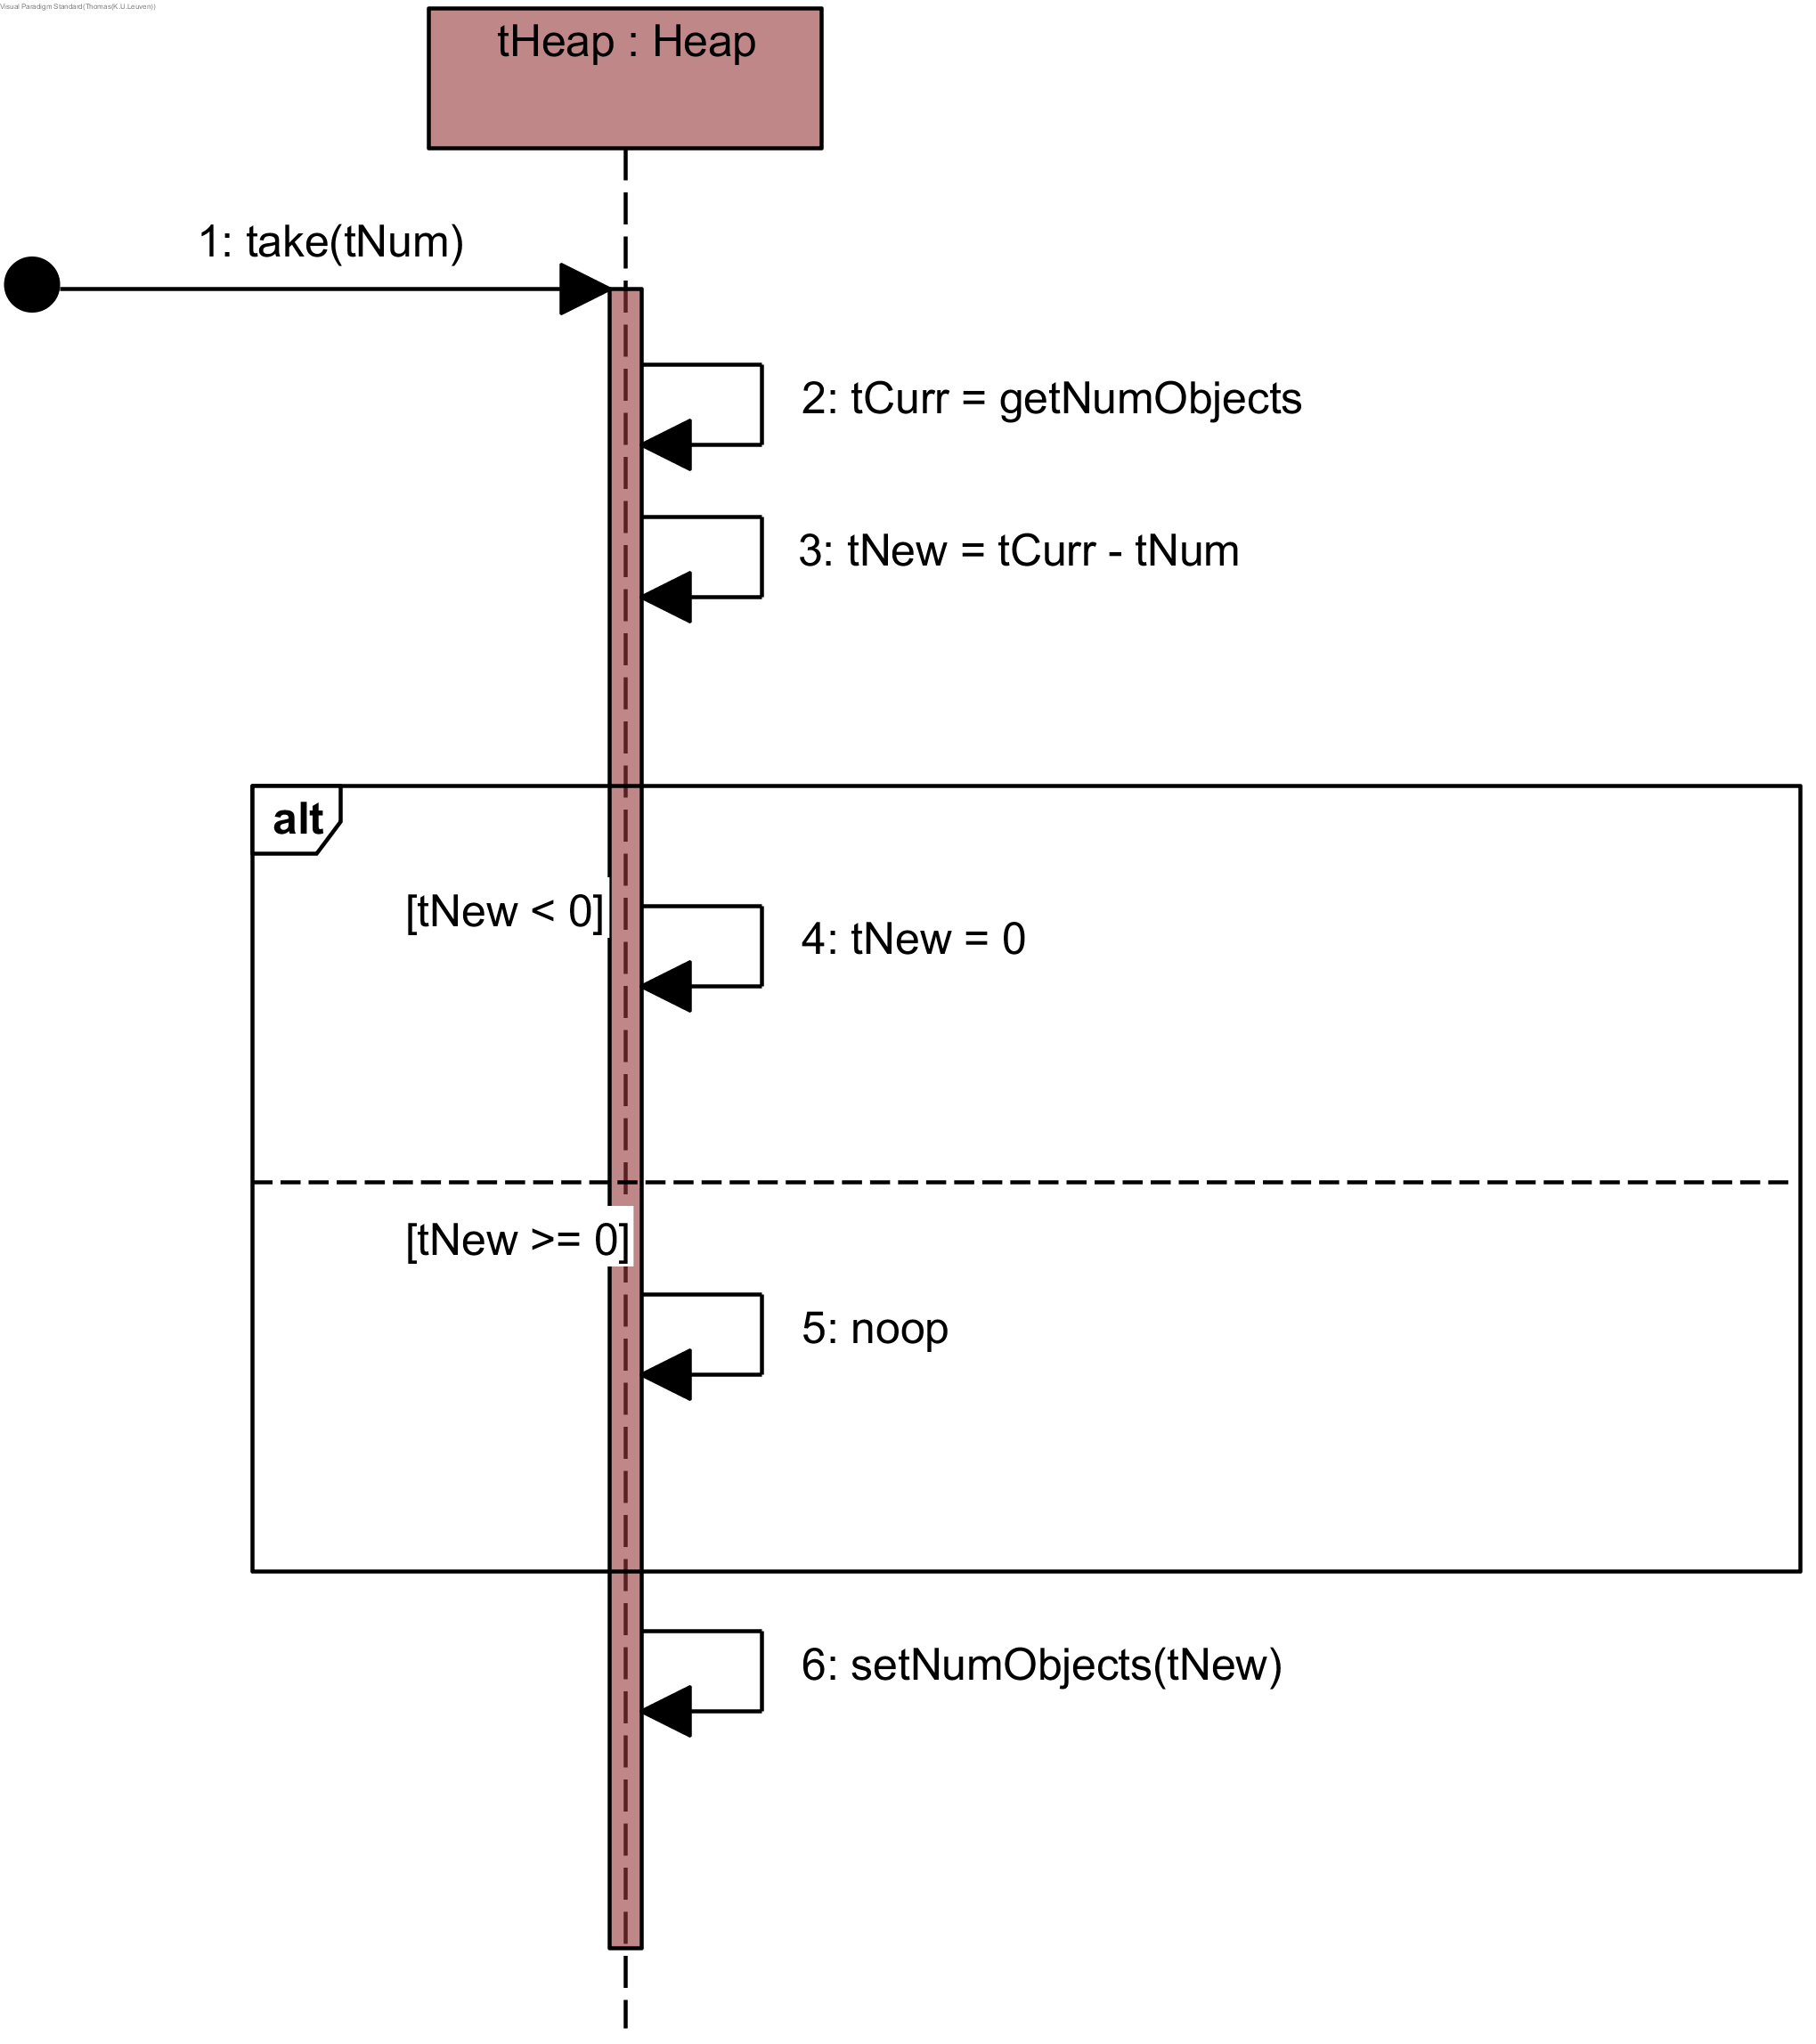
\includegraphics[width=0.8\textwidth]{chap-evaluatie/take.png}
	\caption{Sequentiediagram voor \textit{take(int)}}
	\label{fig:nim-take}
\end{figure}

\subsection{Evaluatie van het ontwerpproces}

Door de beperkingen opgesomd in sectie \ref{sec:beperkingen} zijn er een aantal onintu\"itieve elementen. Als het mogelijk was geweest om de associaties van een object aan te passen tijdens de uitvoering, zou er een klasse \textit{Player} zijn geweest en een associatie \textit{Game}---\textit{Player} die de winnaar aanduidt. Aangezien er maar twee spelers zijn, is het echter voldoende om de winnaar voor te stellen met een booleaanse waarde. Als \textit{gameFinished} waar is, kan toch de winnaar ondubbelzinnig aangeduid worden.

Nim is een simpel spel, dus waren er geen noemenswaardige moeilijkheden bij het ontwerp van de diagrammen. Omdat men maar relatief simpele taken kan doen met \'e\'en enkele instructie, leidt dit er wel toe dat er een veelvoud aan instructies nodig zijn, wat de tijd die nodig is om het ontwerp te maken verhoogt.

\section{Evaluatie van de uitvoertheorie}

Alle testen worden uitgevoerd op een machine die Ubuntu 16.04.3 LTS draait. Deze machine heeft als CPU de Intel(R) Core(TM)2 CPU 6600 en heeft 3969 MB aan geheugen beschikbaar. We gebruiken versie 3.7.0 van IDP.

De volgende testen worden uitgevoerd:

\begin{enumerate}
	\item Simulatie van het verloop van een spel met twee stapels, waarvan \'e\'en twee objecten heeft en de andere drie, door middel van progressie\"inferentie.
	\item Verificatie van de correctheid van het diagram voor \textit{isEmpty()}.
	\item Verificatie van de correctheid van het diagram voor \textit{allHeapsEmpty()}. 
\end{enumerate}

\subsection{Evaluatie van de simulatie}

In deze simulatie neemt de eerste speler tijdens zijn beurt alle drie de objecten van de stapel met drie objecten. Vervolgens neemt de tweede speler \'e\'en object van de andere stapel. Nu heeft de eerste speler geen keuze en moet hij het overblijvend object nemen, waardoor hij het spel verliest.

Figuur \ref{fig:ms} bevat een boxplot van de rekentijd per simulatiestap, en figuur \ref{fig:ms-nooutliers} bevat een boxplot van dezelfde gegevens zonder de uitschieters. We zien dat voor ongeveer de helft van de tijdstappen de rekentijd tussen ongeveer 6,65 seconden en 6,9 seconden ligt. Globaal gezien is de rekentijd gespreid tussen ongeveer 6,5 seconden en 7,15 seconden. Dit zorgt er echter voor dat het ongeveer achttien minuten duurt om het spel volledig uit te spelen. Stap 23, 67 en 111 waren de stappen wanneer de speler een stapel kon kiezen. Het duurde ongeveer twee en een halve minuut om stap 23 te bereiken. Tussen stap 23 en 67 en tussen stap 67 en 111 was er telkens een tijdspanne van ongeveer vijf minuten.

\begin{figure}
	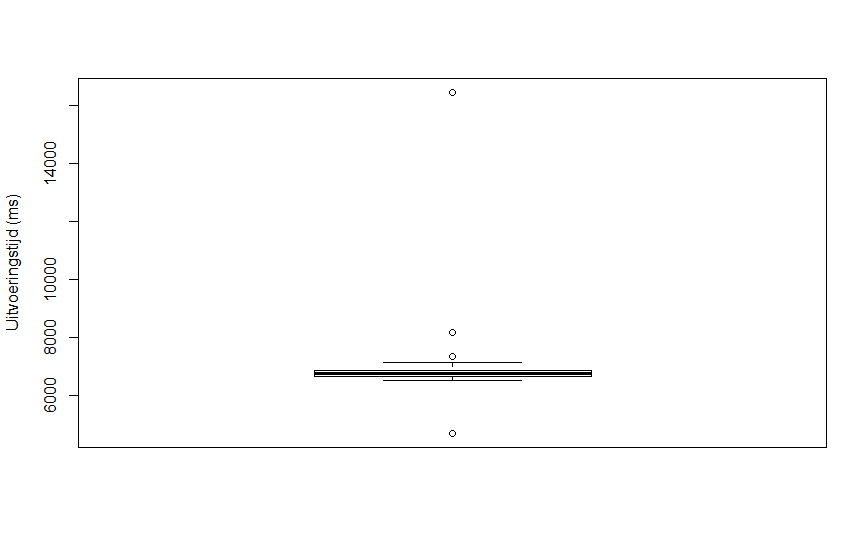
\includegraphics[width=1.05\textwidth]{chap-evaluatie/boxplot.png}
	\caption{Boxplot van de rekentijd per stap}
	\label{fig:ms}
\end{figure}

\begin{figure}
	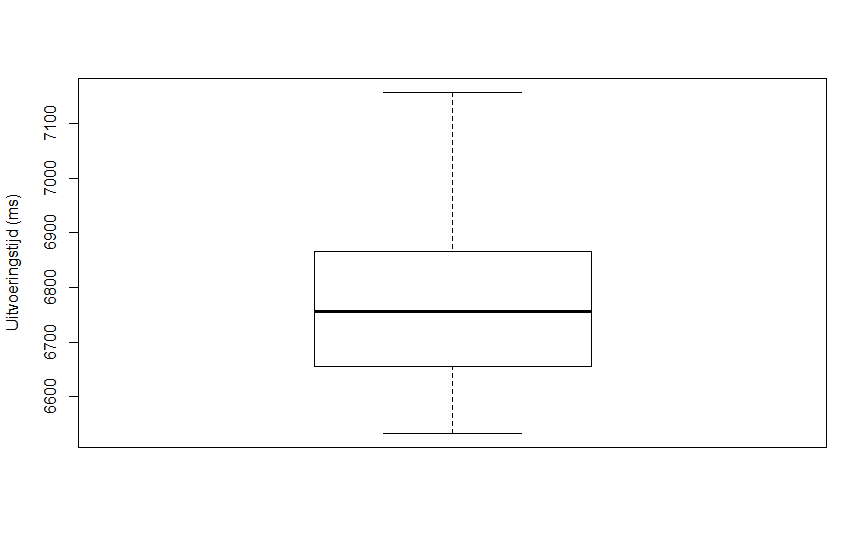
\includegraphics[width=1.05\textwidth]{chap-evaluatie/boxplotnooutliers.png}
	\caption{Boxplot van de rekentijd per stap zonder uitschieters}
	\label{fig:ms-nooutliers}
\end{figure}

Tabel \ref{tab:sim-mem} bevat een overzicht van het virtueel geheugengebruik gemeten aan het begin van elke beurt.


\begin{table}[]
	\centering
	\begin{tabular}{|l|l|l|l|l|}
		\hline
		Beurt 1 & 0,91 GB  \\ \hline
		Beurt 2 & 2,09 GB  \\ \hline
		Beurt 3 & 3,34 GB  \\ \hline
		Einde   & 4,84 GB  \\ \hline
	\end{tabular}
	\caption{Virtueel geheugengebruik aan het begin van elke beurt}
	\label{tab:sim-mem}
\end{table}

Uit deze resultaten blijkt dat we met de uitvoertheorie het spel kunnen spelen, maar het tijdsinterval tussen beurten is groot, en na enkele beurten wordt er al meerdere gigabytes aan virtueel geheugen gebruikt.

\section{Verificatie van de correctheid van \textit{isEmpty()}}

We willen controleren of het diagram in figuur \ref{fig:nim-isEmpty} een positief antwoord geeft als en slechts als de gegeven stapel leeg is. We werken met een invoerstructuur die stelt dat de uitvoering begint met de eerste instructie van \textit{isEmpty} en eindigt na de laatste instructie van hetzelfde diagram. De invoerstructuur specificeert dat er in totaal zeven tijdstappen zijn.

Om de correctheid te controleren stellen we vier zinnen op:

\begin{align}
	\nonumber&\exists{t}[Time]\exists{st}[StackLevel]\exists{h}[Heap]\exists[n][LimitedInt](SDPointAt(t, finished) \\ &\land IeToReturnT(t, st, F) \land HeapamountObjects(t, h, n) \land n \leq 0).\label{form:ie_fnonempty} \\
	\nonumber&\exists{t}[Time]\exists{st}[StackLevel]\exists{h}[Heap]\exists[n][LimitedInt](SDPointAt(t, finished) \\ &\land IeToReturnT(t, st, T) \land HeapamountObjects(t, h, n) \land n > 0).\label{form:ie_fempty} \\
	\nonumber&\exists{t}[Time]\exists{st}[StackLevel]\exists{h}[Heap]\exists[n][LimitedInt](SDPointAt(t, finished) \\ &\land IeToReturnT(t, st, T) \land HeapamountObjects(t, h, n) \land n \leq 0).\label{form:ie_cempty} \\
	\nonumber&\exists{t}[Time]\exists{st}[StackLevel]\exists{h}[Heap]\exists[n][LimitedInt](SDPointAt(t, finished) \\ &\land IeToReturnT(t, st, F) \land HeapamountObjects(t, h, n) \land n > 0).\label{form:ie_cnonempty}
\end{align}

Zin \ref{form:ie_fnonempty} schrijft voor dat het antwoord negatief is, maar dat de stapel nul of minder objecten heeft.

Zin \ref{form:ie_fempty} is gelijkaardig, maar controleert op een positief antwoord met een stapel met meer dan nul objecten.

Beide zinnen moeten leiden tot een onvervulbare theorie.

Zin \ref{form:ie_cempty} schrijft voor dat het antwoord positief is en dat de stapel nul of minder objecten heeft.

Zin \ref{form:ie_cnonempty} controleert op een negatief antwoord met een stapel met meer dan nul objecten.

Beide zinnen moeten leiden tot een vervulbare theorie.

We voeren IDP viermaal uit met de voorgaande zinnen om de beurt toegevoegd aan de invoertheorie. Voor de twee eerste zinnen krijgen we inderdaad als antwoord dat de theorie onvervulbaar is. Voor zin \ref{form:ie_cempty} krijgen we een uniek model dat overeenkomt met een lege stapel. Voor zin \ref{form:ie_cnonempty} krijgen we alle modellen met een stapel die niet leeg is.

Er is een gelijkaardig tijdsverloop en \textit{grounding}-grootte voor alle vier de uitvoeringen. Het duurt ongeveer 29 seconden en de \textit{grounding}-grootte is 578 306. We duiden deze cijfers in de volgende sectie.

We merken op dat het relatief lang duurt om modelexpansie uit te voeren voor dit diagram. De \textit{grounding} is ook omvangrijk.

\section{Verificatie van de correctheid van \textit{allHeapsEmpty()}}

We willen controleren of het diagram in figuur \ref{fig:nim-allHeapsEmpty} een positief antwoord geeft als alle stapels leeg zijn en een negatief antwoord als minstens \'e\'en stapel niet leeg is. We werken met een invoerstructuur die aangeeft dat de uitvoering begint met de eerste instructie van \textit{allHeapsEmpty} en eindigt na de laatste instructie van dat diagram. De invoerstructuur specificeert dat er in totaal 22 tijdstappen zijn.

We stellen vier zinnen op:

\begin{align}
	\nonumber&\exists{t}[Time]\exists{st}[StackLevel](SDPointAt(22, allHeapsEmpty\_8) \\ &\land \lnot\exists{h}[Heap]\exists{n}[LimitedInt](HeapamountObjects(t, h, n) \land n > 0)).\label{form:ahe_fnonempty} \\
	\nonumber&\exists{t}[Time]\exists{st}[StackLevel]\exists{h}[Heap]\exists[n][LimitedInt] \\ &(SDPointAt(22, allHeapsEmpty\_7) \land HeapamountObjects(t, h, n) \land n > 0).\label{form:ahe_fempty} \\
	\nonumber&\exists{t}[Time]\exists{st}[StackLevel](SDPointAt(22, allHeapsEmpty\_7) \\ &\land \forall{h}[Heap]\forall{n}[LimitedInt](HeapamountObjects(t, h, n) \Rightarrow n \leq 0)).\label{form:ahe_cempty} \\
	\nonumber&\exists{t}[Time]\exists{st}[StackLevel]\exists{h}[Heap]\exists[n][LimitedInt] \\ &(SDPointAt(22, allHeapsEmpty\_8) \land HeapamountObjects(t, h, n) \land n > 0).\label{form:ahe_cnonempty}
\end{align}

We benoemen expliciet tijdstap 22 omdat de machine net voldoende geheugen heeft om modelexpansie uit te voeren met dat aantal tijdstappen. 22 tijdstappen zijn voldoende om gegeven twee stapels een punt te bereiken in het diagram waarop het antwoord eigenlijk al bekend is. Instructie 7 komt overeen met het geval waar het antwoord positief is; instructie 8 komt overeen met het geval waar het antwoord negatief is.

Zin \ref{form:ahe_fnonempty} stelt voor dat het antwoord negatief is, maar dat er geen stapel bestaat met meer dan nul objecten.

Zin \ref{form:ahe_fempty} stelt voor dat het antwoord positief is, maar dat er een stapel bestaat met meer dan nul objecten.

Deze twee zinnen moeten leiden tot de conclusie dat de theorie onvervulbaar is.

Zin \ref{form:ahe_cempty} stelt voor dat het antwoord positief is en dat alle stapels leeg zijn.

Zin \ref{form:ahe_cnonempty} stelt voor dat het antwoord negatief is en dat er een stapel bestaat met meer dan nul objecten.

De conclusie moet hier zijn dat de theorie vervulbaar is.

Wanneer we IDP viermaal runnen met deze vier zinnen om de beurt toegevoegd aan de uitvoertheorie, is de theorie inderdaad onvervulbaar voor de eerste twee zinnen. Zin \ref{form:ahe_cempty} leidt tot een uniek model dat overeenkomt met het geval dat alle stapels leeg zijn. Zin \ref{form:ahe_cnonempty} geeft alle modellen waar minstens \'e\'en stapel meer dan nul objecten heeft.

De uitvoeringstijd en \textit{grounding}-grootte zijn gelijkaardig voor alle vier uitvoeringen. De uitvoering duurt ongeveer 1 minuut en 28 seconden en de \textit{grounding}-grootte is 2 249 098.

Ter vergelijking duurt het voor de theorie in bijlage \ref{app:new-nim} dat overeenkomt met het diagram in figuur \ref{fig:new-nim} ongeveer 31,6 seconden om alle modellen te vinden voor een volledig spelverloop met twee stapels, waarbij \'e\'en stapel twee objecten heeft en de andere drie. De \textit{grounding}-grootte is daarbij 142 510. De invoerstructuur voor deze uitvoering specificeert dat er in totaal 100 tijdstappen zijn.

\subsection{Samenvatting van de bevindingen}
Men kan Nim spelen met de theorie die automatisch werd gegenereerd uit de gegeven diagrammen. Tussen elke beurt is er wel een wachttijd van ongeveer vijf minuten, met twee en een halve minuut voordat de eerste beurt gespeeld kan worden.

Het is mogelijk om voor een diagram bepaalde gewenste eigenschappen te controleren. Dit gaat echter gepaard met grote \textit{groundings} en een lange uitvoeringstijd. Bijgevolg konden we niet controleren welke uitvoerpaden er bestaan die ertoe leiden dat een bepaalde speler wint beginnend van een bepaald scenario.

Dit leidde er ook toe dat we ons initieel evaluatiescenario niet konden uitvoeren. Hierbij keken we naar het spel Reversi, wat een bordspel voor twee spelers is. E\'en speler is wit en de andere speler is zwart. Wanneer het spel begint, liggen er al twee witte schijven en twee zwarte schijven. Zwart begint. De spelers leggen om de beurt een schijf op een lege plek. Alle schijven van de tegenspeler die tussen de pas gelegde schijf en een andere schijf van de speler die aan zet is liggen, veranderen van kleur. Als de speler geen zet kan doen waardoor er minstens \'e\'en schijf van de tegenspeler van kleur verandert, slaat hij zijn beurt over. Het spel eindigt als er twee beurten moeten overgeslagen worden. De speler met de meeste schijven op het veld die zijn kleur hebben wint.

We hebben voor dit spel ook een klassediagram en een stel van elf sequentiediagrammen ontworpen. Onze software kon deze diagrammen vertalen naar een FO($\cdot$)-theorie, maar de rekentijd en het geheugengebruik waren zo groot dat het niet lukte om \'e\'en beurt te simuleren.